\subsection{摩擦・不感帯・バックラッシの測定と補償}

電流制限と電圧制限を考慮すると、指令がアクチュエータの許容範囲を越えないようにできる。
しかし、許容範囲内の小さな指令が、そのまま小さな運動になるとは限らない。
DC モータをギヤで減速した位置サーボでは、低速で止まりかけたときに静止摩擦が効き、ドライバや機構の不感帯によって小さな電圧指令が出力へ届かず、回転方向を反転した直後にはギヤのバックラッシを詰めるまで負荷側が遅れる。
したがって、前段までの飽和対策で
\[
  |v|\leq V_{\max},\qquad |\tau_c|\leq \tau_{\max}
\]
を守っていても、測定された負荷角 $\theta_l$ は目標角 $\theta_{l,r}$ に追従しない場合がある。
ここで $v$ はモータドライバへの電圧指令 $[\mathrm{V}]$、$\tau_c$ は電流ループまたはトルク制御器が作るモータ軸トルク指令 $[\mathrm{N\,m}]$、$\omega$ はモータ角速度 $[\mathrm{rad/s}]$、$\theta_m$ はモータ軸角 $[\mathrm{rad}]$、$\theta_l$ は負荷側角 $[\mathrm{rad}]$ である。

以下では、内側の電流ループは外側の位置ループより十分速く、低速域では温度と荷重が短時間で大きく変わらないと仮定する。
また、軸の弾性変形はバックラッシ幅に比べて小さく、摩擦・不感帯・バックラッシは一軸の測定曲線として扱えるとする。
この仮定は補償式を作るための近似であり、摩擦やすきまを物理的に消す仮定ではない。

\subsubsection{低速掃引による非線形特性の測定}

まず、負荷を外さずに低速で正負方向へ掃引し、静止摩擦、動摩擦、不感帯、バックラッシを別々に測る。
\wfig{friction-deadzone-backlash-examples} は、次の数値を持つ小形 DC モータサーボの低速測定例である。
\[
  \tau_s=0.16\,\mathrm{N\,m},\qquad
  \tau_k=0.105\,\mathrm{N\,m},\qquad
  b=0.018\,\mathrm{N\,m\,s/rad},
\]
\[
  v_d=0.72\,\mathrm{V},\qquad
  K_v=8.0\,\mathrm{rad/(s\,V)},\qquad
  \Delta_\theta=0.18\,\mathrm{rad}.
\]
$\tau_s$ は止まっている軸を動かし始めるための静止摩擦トルク、$\tau_k$ は動き始めた後の Coulomb 摩擦トルク、$b$ は粘性摩擦係数、$v_d$ は不感帯の片側幅、$K_v$ は不感帯を越えた後の低速ゲイン、$\Delta_\theta$ は負荷側に現れるバックラッシ幅である。

低速で一定角速度 $\omega$ を保つために必要なトルクを測ると、動いている範囲では
\[
  \tau_{\mathrm{meas}}(\omega)
  \simeq b\omega+\tau_k\operatorname{sgn}(\omega),
  \qquad \omega\neq 0
\]
と近似できる。
一方、静止中は一つの値ではなく区間として扱う。
外乱トルクを含めた駆動側の差し引きトルクが
\[
  -\tau_s \leq \tau_{\mathrm{drive}}-\tau_{\mathrm{load}}\leq \tau_s
\]
に入ると、角速度は $\omega=0$ のままになり得る。
このため、比例制御器が小さな偏差から小さなトルクを作っても、そのトルクが静止摩擦帯の内側なら運動は始まらない。

ドライバの不感帯は、電圧指令 $v$ と定常角速度 $\omega_{\mathrm{ss}}$ の測定から
\[
  \omega_{\mathrm{ss}}(v)
  \simeq
  K_v\operatorname{sgn}(v)\max\{|v|-v_d,0\}
\]
と近似する。
この式は、$|v|\leq v_d$ では電圧指令を変えても定常角速度がほぼ 0 であり、$|v|>v_d$ になってから傾き $K_v$ の直線に近づくことを表す。
電圧制限 $|v|\leq V_{\max}$ を守っていても、$v_d$ より小さい指令しか出ていないなら、実機には入力が入っていないのと同じ状態が生じる。

バックラッシは、モータ軸をゆっくり往復させて、モータ軸角 $\theta_m$ と負荷側角 $\theta_l$ の閉じない曲線として測る。
単純なすきまモデルでは、接触面が正転側に当たっているとき
\[
  \theta_l\simeq \theta_m-\frac{\Delta_\theta}{2},
\]
逆転側に当たっているとき
\[
  \theta_l\simeq \theta_m+\frac{\Delta_\theta}{2}
\]
である。
その間の区間では、モータ軸だけが動いても負荷側がまだ動かない。
方向反転の直後に負荷角の応答が遅れるのは、このすきまを詰める運動が先に必要になるためである。

\subsubsection{逆特性を用いた補償入力}

補償では、測定した非線形特性の逆向きの入力を、線形フィードバックの外側または前置補償として加える。
符号関数をそのまま使うとゼロ付近で入力が急に切り替わり、量子化やノイズで微小振動を起こしやすい。
そこで
\[
  \sigma_\epsilon(x)=\tanh\left(\frac{x}{\epsilon}\right)
\]
を滑らかな符号近似として使う。
速度目標 $\omega_r$ に対する摩擦補償トルクは
\[
  \tau_{\mathrm{fric}}(\omega_r)
  =b\omega_r+\tau_k\sigma_{\epsilon_\omega}(\omega_r)
\]
と置ける。
線形制御器が作る等価電圧を $v_\ell$ とし、モータトルク定数を $K_t\,[\mathrm{N\,m/V}]$ とまとめて表すと、不感帯と摩擦を含む電圧補償は
\[
  v_c
  =
  \operatorname{sat}_{[-V_{\max},\,V_{\max}]}
  \left(
    v_\ell
    +v_d\sigma_{\epsilon_v}(v_\ell)
    +\frac{\tau_{\mathrm{fric}}(\omega_r)}{K_t}
  \right)
\]
である。
飽和関数 $\operatorname{sat}_{[-V_{\max},\,V_{\max}]}(\cdot)$ は、補償を加えた後でも電圧制限を越えないために残しておく。
補償項が大きすぎて飽和に当たる場合、静止摩擦や不感帯の一部は補えず、前節までの制限が再び支配的になる。

バックラッシは、目標負荷角 $\theta_{l,r}$ に対して、接触させたい側へモータ軸目標を先にずらす。
負荷側の目標速度を $\dot{\theta}_{l,r}$ とすると、
\[
  \theta_{m,r}^{\mathrm{comp}}
  =
  \theta_{l,r}
  +\frac{\Delta_\theta}{2}
  \sigma_{\epsilon_\theta}(\dot{\theta}_{l,r})
\]
である。
正転中はモータ軸目標を負荷側目標より $\Delta_\theta/2$ だけ進め、逆転中は同じ量だけ戻す。
この補償は、どちらの歯面へ接触させたいかをあらかじめ決める操作であり、負荷側がすきまの中で自由に動く瞬間を完全にはなくせない。

\begin{figure}[tbp]
\centering
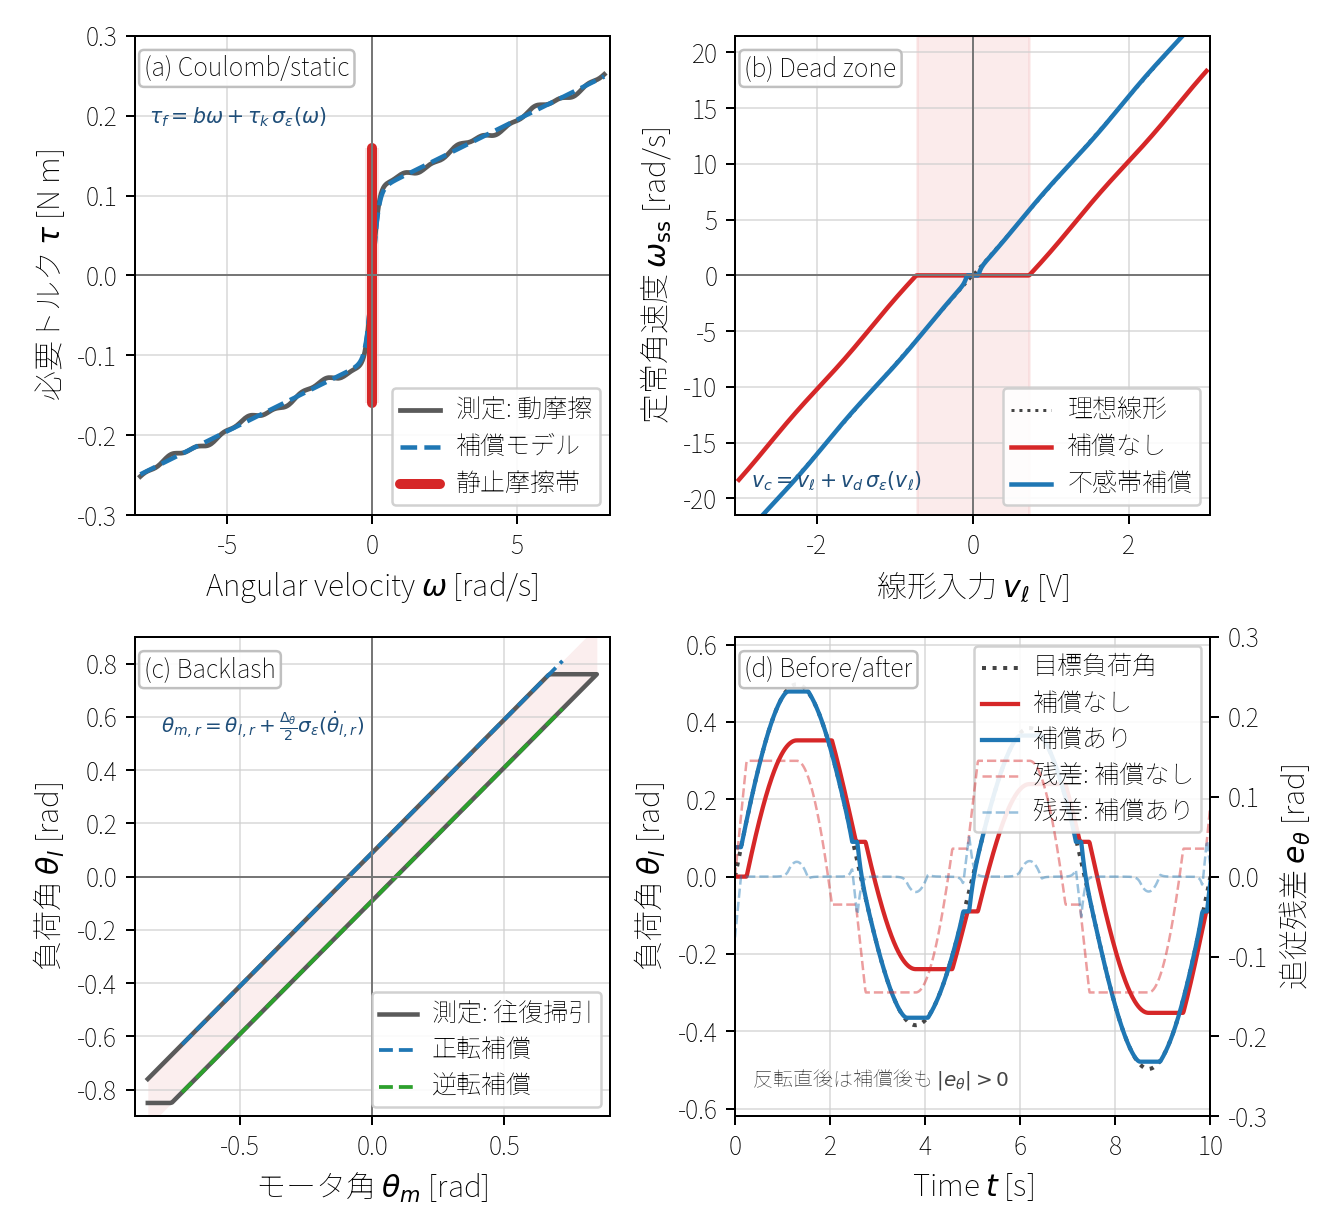
\includegraphics[width=0.96\linewidth,bb=0 0 1332 1224]{figures/friction_deadzone_backlash_examples.png}
\caption{摩擦・不感帯・バックラッシの低速測定曲線と補償例。左上は静止摩擦帯と Coulomb 摩擦を含む必要トルク、右上は不感帯を持つ電圧-角速度特性と逆向きの電圧補償、左下は往復掃引で得られるバックラッシ曲線と接触側を選ぶ角度補償、右下は反転を含む負荷角追従の補償前後である。補償後も反転直後の残差は残り、これはすきまを詰める時間と摩擦変動が残るためである。}
\label{fig:friction-deadzone-backlash-examples}
\end{figure}

\subsubsection{補償後に残る限界}

\wfig{friction-deadzone-backlash-examples} の右下では、不感帯とバックラッシを補償しない場合、目標負荷角が小さく変わっても出力が止まり、方向反転後に負荷側の動き出しが遅れている。
補償を入れると、小さな目標変化でも不感帯を越える入力が作られ、反転時にはモータ軸目標が先にずれるため、追従残差は小さくなる。
ただし、残差は 0 にはならない。
理由は三つある。

第一に、静止摩擦は荷重、温度、潤滑状態、停止時間で変わる。
測定値 $\tau_s$ を少し大きめに補償すると止まりにくくなるが、大きすぎると目標近傍で正負に入力が切り替わり、微小な往復運動を作る。
第二に、不感帯幅 $v_d$ はドライバ、電源電圧、PWM 分解能、機械抵抗によって変わる。
補償式の $v_d$ は一定値ではなく、実装では温度や速度範囲ごとに表を切り替える場合がある。
第三に、バックラッシは接触していない区間では負荷側の位置を拘束しない。
反転直後に幅 $\Delta_\theta$ のすきまを詰めるには、少なくとも
\[
  t_{\mathrm{takeup}}
  \gtrsim
  \frac{\Delta_\theta}{|\dot{\theta}_m|}
\]
の時間が必要である。
電圧制限や速度制限によって $|\dot{\theta}_m|$ が上げられないと、この遅れは補償式だけでは消えない。

したがって、摩擦・不感帯・バックラッシ補償は完全な相殺ではなく、測定した失われる入力範囲を先に越えるための前置補償である。
線形フィードバックは補償後にも必要であり、残る誤差、温度変化、モデル誤差、飽和時の切り詰めを吸収する役割を持つ。
次の段階で速度・加速度の目標値から単純なフィードフォワードを加えるときも、ここで扱った補償項と飽和条件を同時に見る必要がある。
